\chapter{Entwicklung einer mobilen Anwendung}
Auf Basis der ausgearbeiteten Ergebnisse aus Kapitel
\ref{chapter:motion-detection} soll nun eine mobile Anwendung entwickelt werden.
Ziel ist es die theoretischen Schlussfolgerungen mit einem praktischen
Experiment zu verifizieren. Da sich diese Arbeit vor allem mit dem Problem
beschäftigen soll, wie solche Modelle auf mobilen Plattformen überführt werden
können, soll eine Android-App entwickelt werden, um die Ergebnisse
zusammenzufassend zu präsentieren. Android wird als Plattform gewählt, da es zur
Zeit die am häufigsten vertretene mobile Plattform ist und ein entsprechendes
Gerät leicht zur Verfügung steht. Zum Vergleich, Android besitzt einen
Marktanteil von 72,84\%, iOS einen von 26,34\% und 0,82\% werden von sonstigen
Plattformen
gehalten\footnote{https://www.statista.com/statistics/272698/global-market-share-held-by-mobile-operating-systems-since-2009/
(besucht am 13.08.2021)}.

Die Anforderungen an die App sind recht simpel. Es sollen über die Kamera
Bewegungen identifiziert werden, wobei die erkannte Bewegungsart angezeigt
werden soll. Das Zeitfenster, in welches Bewegungen erkannt werden sollen, wird
auf 60 Frames festgelegt. Bei einer Kamera, die 30 Bilder pro Sekunde aufnehmen
kann, wird also vorausgesetzt, dass die Bewegung innerhalb von zwei Sekunden
eindeutig identifizierbar ist. Zusätzlich muss berücksichtigt werden, dass die
Abtastrate für die Bewegungserkennung entsprechend hoch, also die
Ausführungsdauer der Machine-Learning-Modelle möglichst gering sein soll. Der
Grund dafür ist, dass die Modelle den Flaschenhals der Anwendung darstellen und
eine hohe Abtastrate nur mit entsprechend schnellen Netzwerken möglich ist.

\section{Implementierungsdetails}
Der Einfachheit halber werden zwei KNNs verwendet, um eine Bewegung zu
identifizieren. Das eine Netzwerk hat die Aufgabe, Schlüsselpunkte des
menschlichen Körpers in Bildern zu erkennen. Diese werden anschließend in einen
Puffer mit maximal 60 Elementen zwischengespeichert. Wird ein Element in den
Puffer hinzugefügt, so werden alle anderen Elemente zuerst um eine Position nach
hinten (rechts) verschoben. Der erste Slot ist nun dementsprechend leer und wird
von dem neuen Element belegt. Ist der Puffer bereits voll, so wird das letzte
Element entfernt. Ein Element dieses Puffers sind 17 Schlüsselpunkte des
menschlichen Körpers. Dieser Puffer bildet damit die Eingabe für das zweite
Netzwerk.  Dieses hat die Aufgabe, Schlüsselpunkte aus 60 Kamerabildern einer
Bewegungsklasse zuzuordnen.

Für die Schlüsselpunkterkennung wird MoveNets Lightning-Architektur
\cite{movenet} verwendet. Diese wurde speziell für mobile Geräte entwickelt,
sodass die Erkennung von Schlüs\-sel\-punk\-ten in Echtzeit durchgeführt werden
kann. Hier gilt es zu testen, ob die Performance in der Tat ausreichend ist, um
auf modernen, aber leistungsärmeren Geräten in Echtzeit zu laufen. Für die
Bewegungserkennung werden die verschiedenen Architekturen aus Kapitel
\ref{chapter:motion-detection} verwendet und getestet. Auch hier ist zu
überprüfen, ob diese in Zusammenarbeit mit MoveNet zu einer ausreichenden
Performance kommen. Eine ausreichende Performance wird dann angenommen, wenn
entsprechende Bewegungen über die Kamera bzw. über die entwickelte App richtig
erkannt wurden.

\begin{figure}
    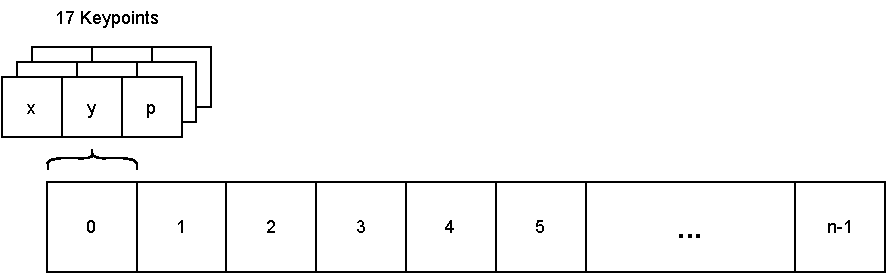
\includegraphics[width=\textwidth]{images/camera_frame_buffer.pdf}
    \caption{Schematische Darstellung des Puffers der Bewegungserkennung,
    welcher $n = 60$ Schlüsselpunkte des menschlichen Körpers speichert.}
\end{figure}

\begin{figure}
    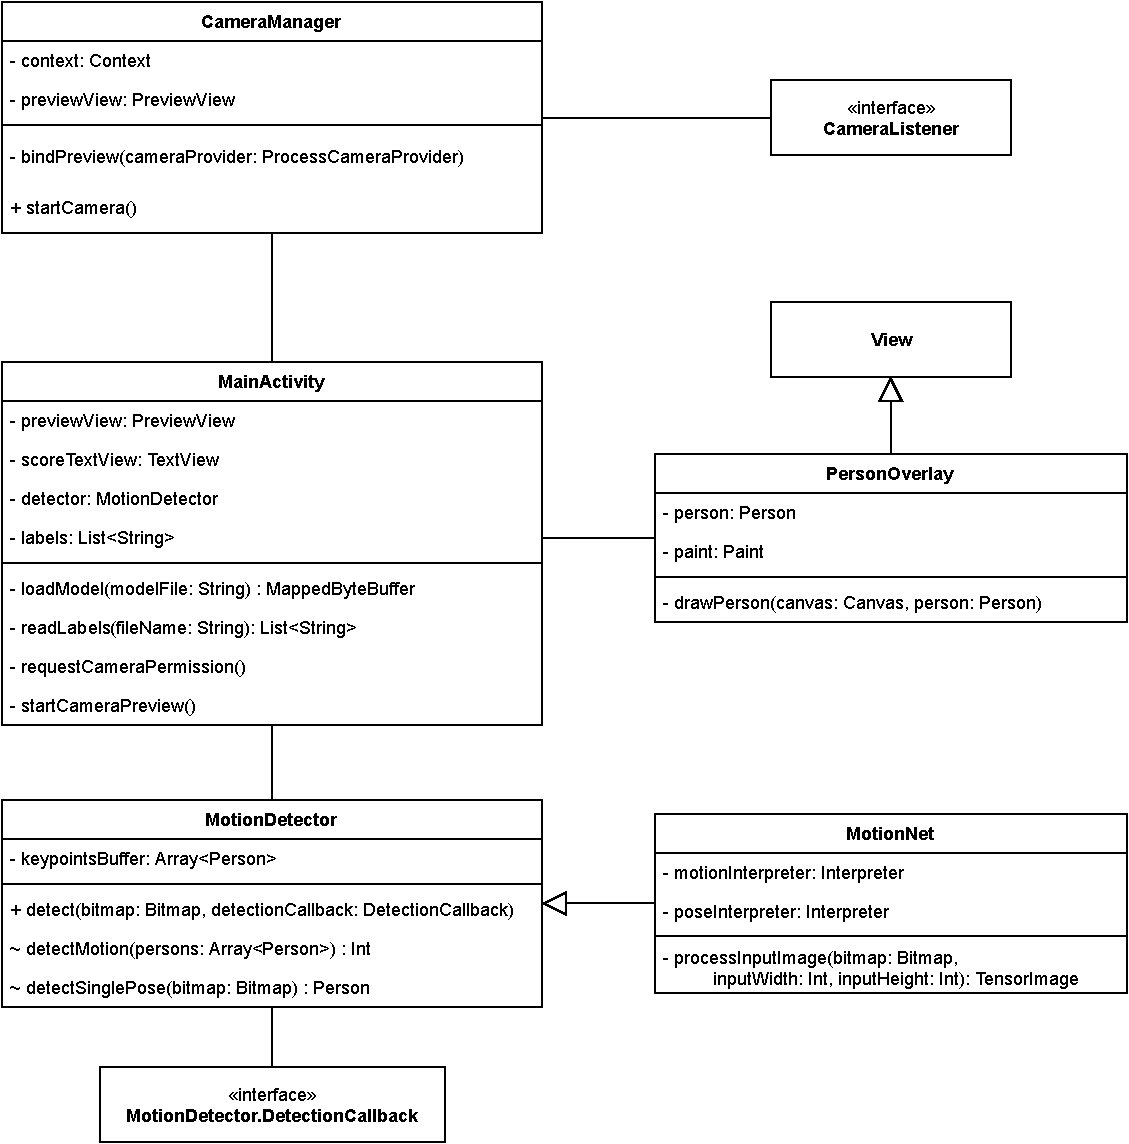
\includegraphics[width=\textwidth]{images/app_uml.pdf}
    \caption{UML-Klassendiagramm der mobilen Anwendung zum Testen der
    Machine-Learning-Modelle für die Bewegungserkennung.}
\end{figure}

